\section{Теоретическая часть}

\subsection{Алгоритм MD5}

На рисунках \ref{img:md5_base}--\ref{img:md5_step} представлена общая схема реализации алгоритма хеширования MD5.

\begin{figure}[!htb]\centering
	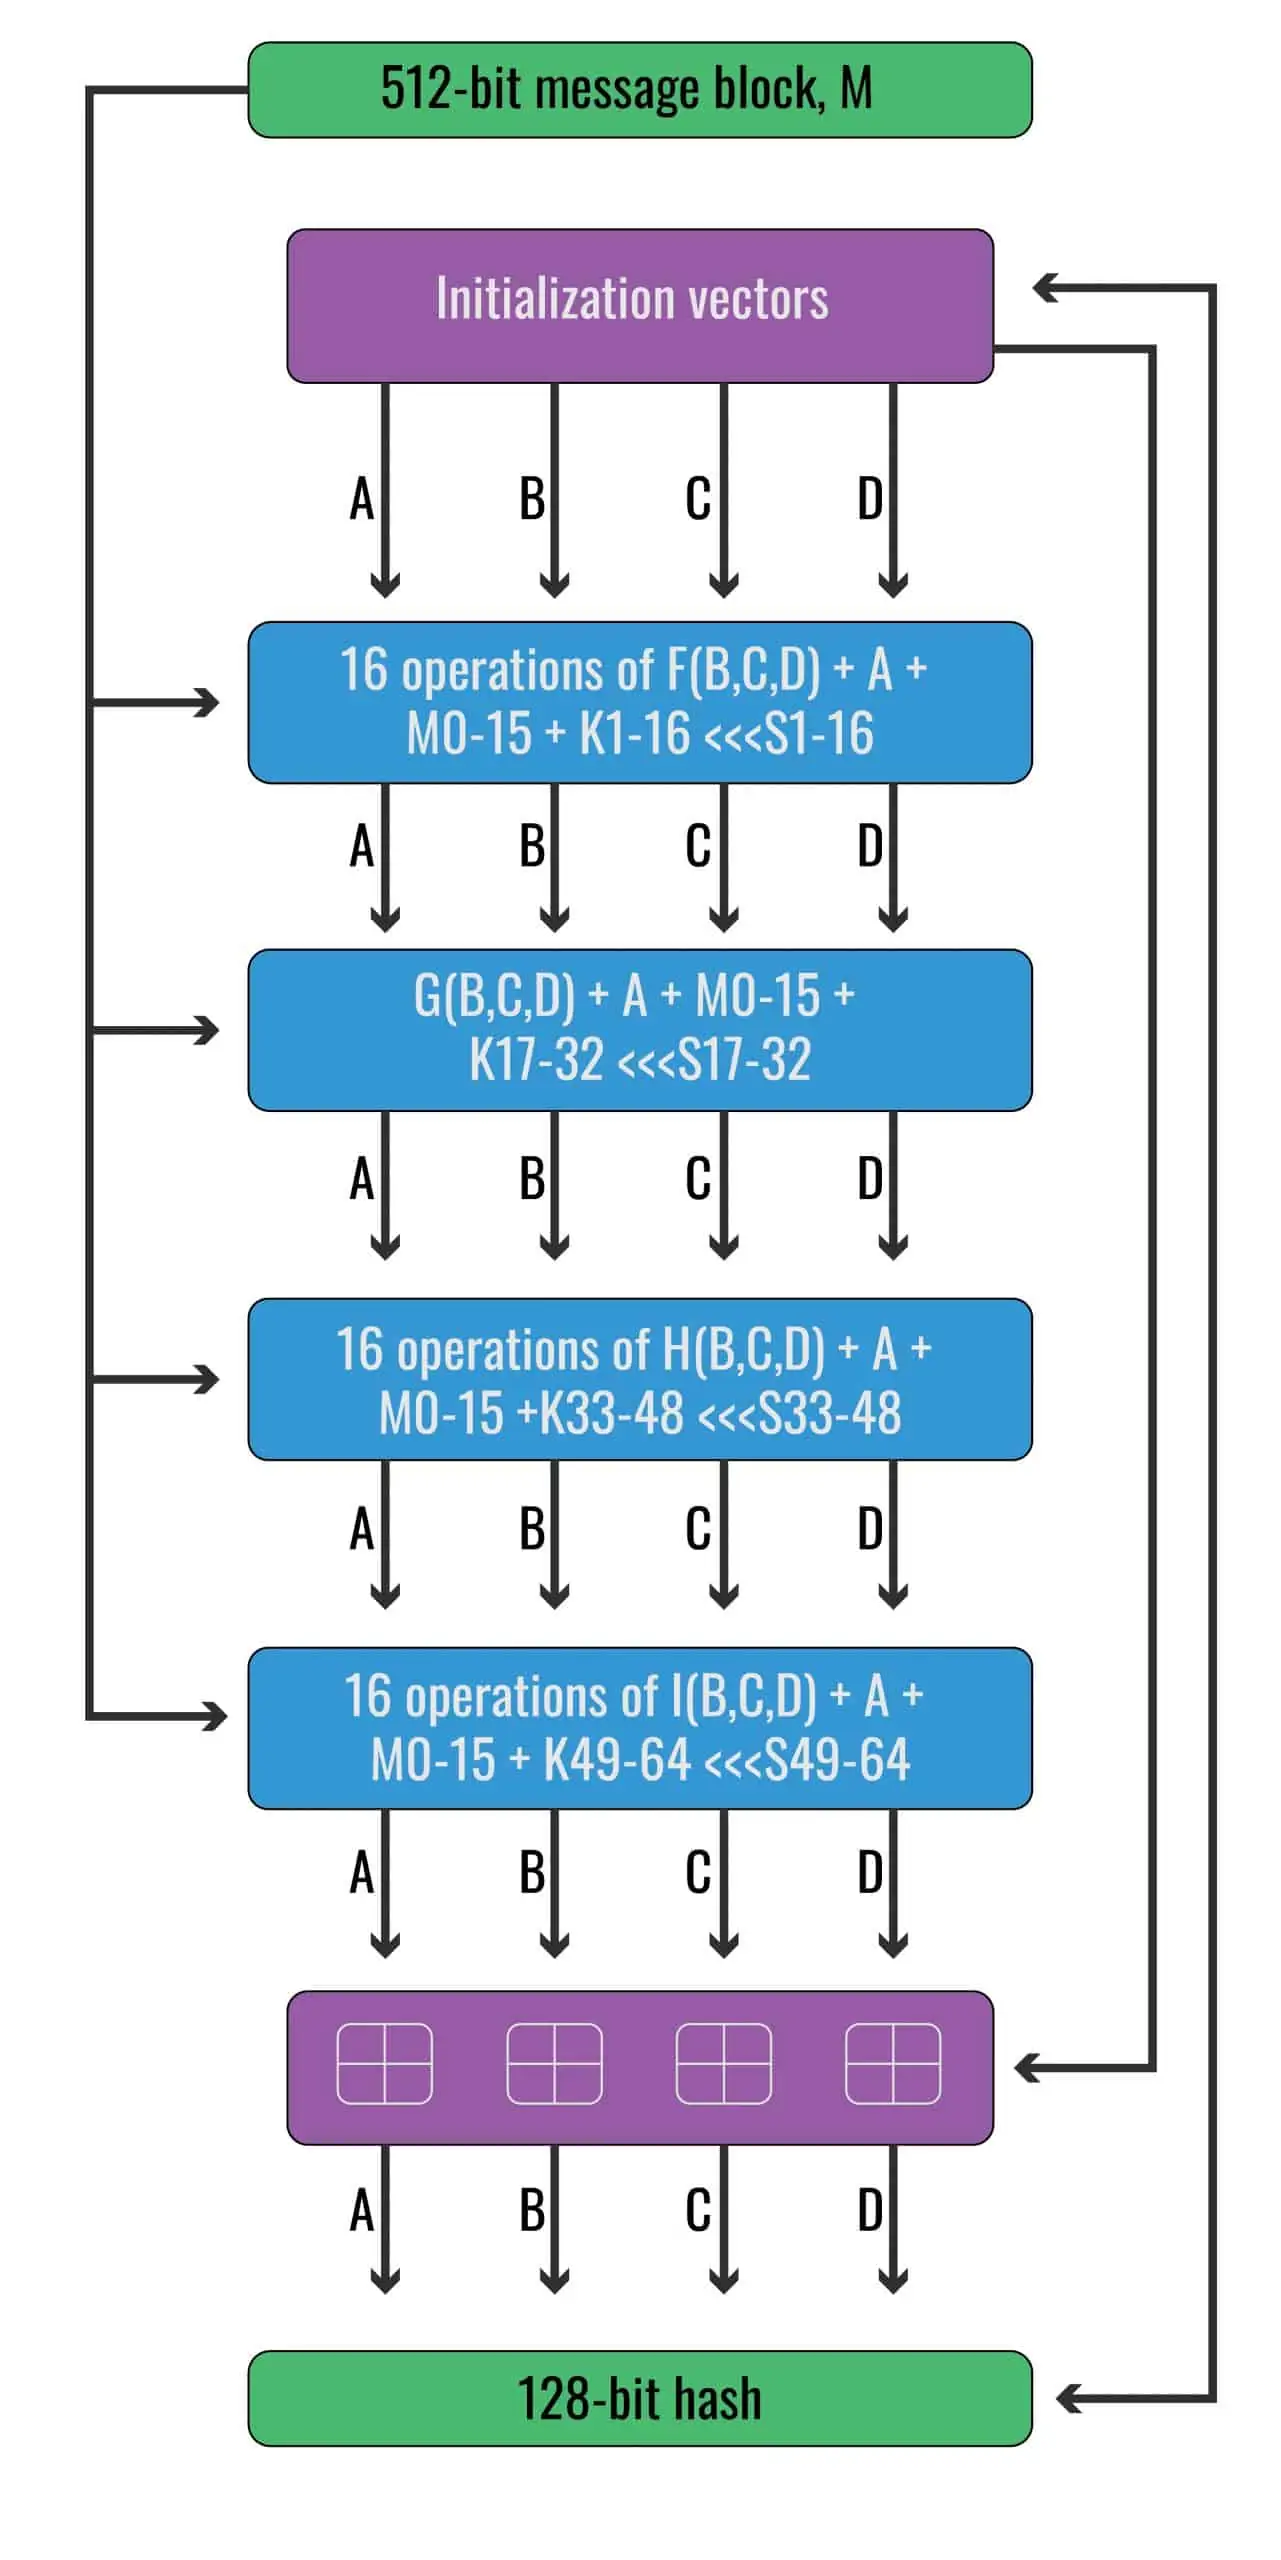
\includegraphics[width=0.45\linewidth]{../img/md5_base.png}
	\caption{Общая схема реализации алгоритма хеширования MD5}
	\label{img:md5_base}
\end{figure}

\newpage

\begin{figure}[!htb]\centering
	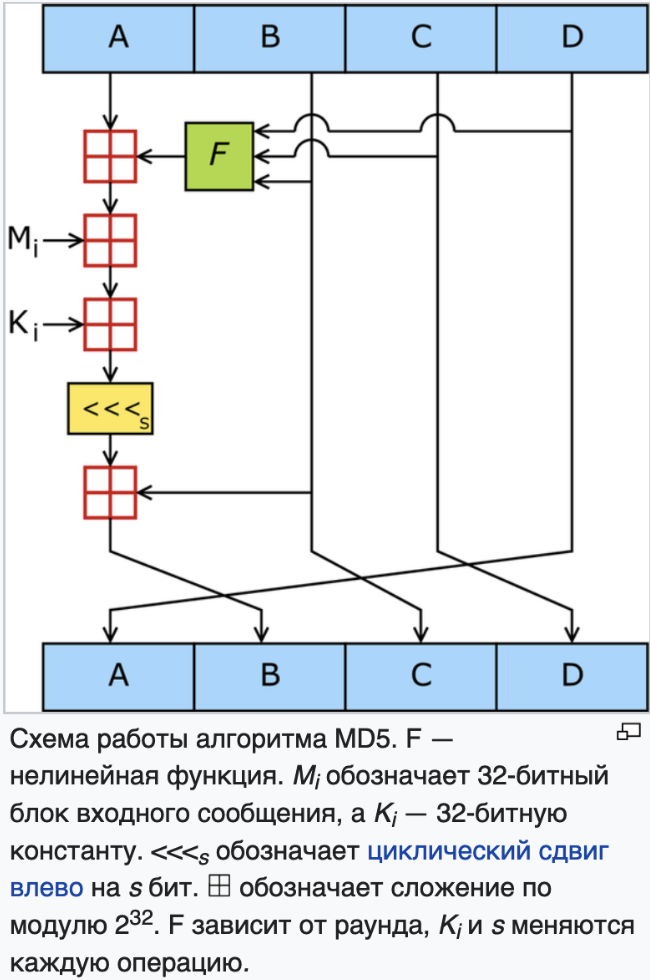
\includegraphics[width=0.45\linewidth]{../img/md5_step.png}
	\caption{Схема реализации алгоритма хеширования MD5}
	\label{img:md5_step}
\end{figure}

\subsection{Алгоритм RSA}
На рисунках \ref{img:rsa}--\ref{img:rsa_keygen} представлена общая схема реализации алгоритма шифрования RSA.

\begin{figure}[!htb]\centering
	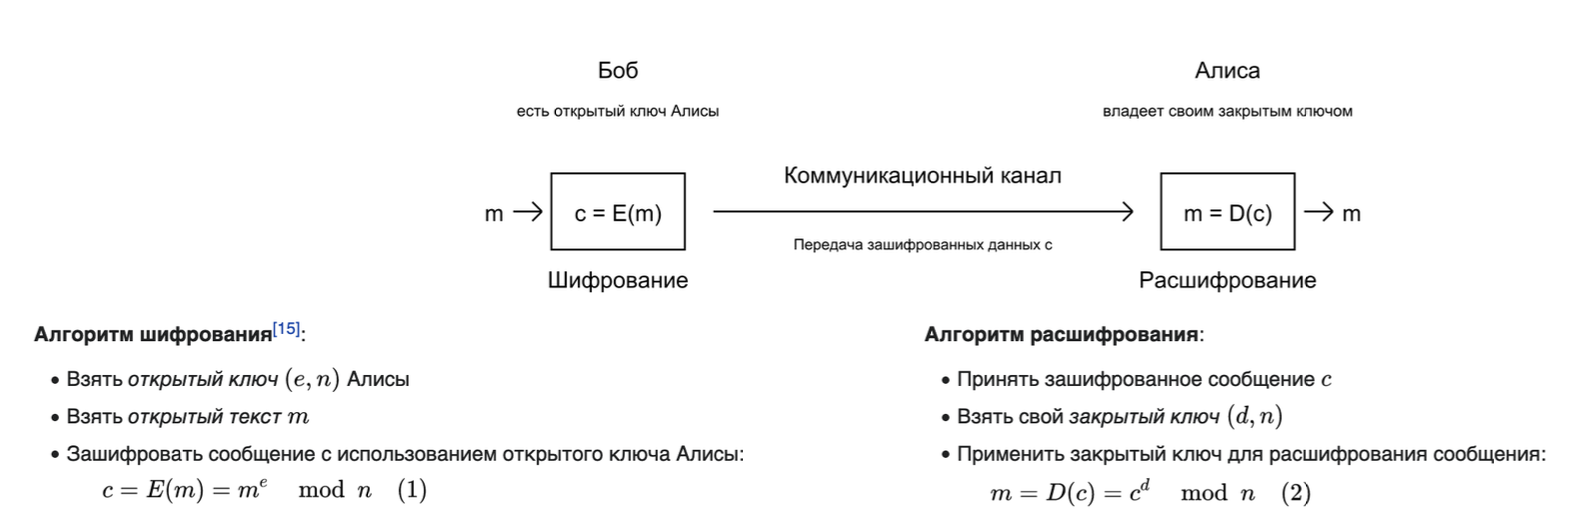
\includegraphics[width=1.0\linewidth]{../img/rsa.png}
	\caption{Общая схема реализации алгоритма шифрования RSA}
	\label{img:rsa}
\end{figure}

\newpage

\begin{figure}[!htb]\centering
	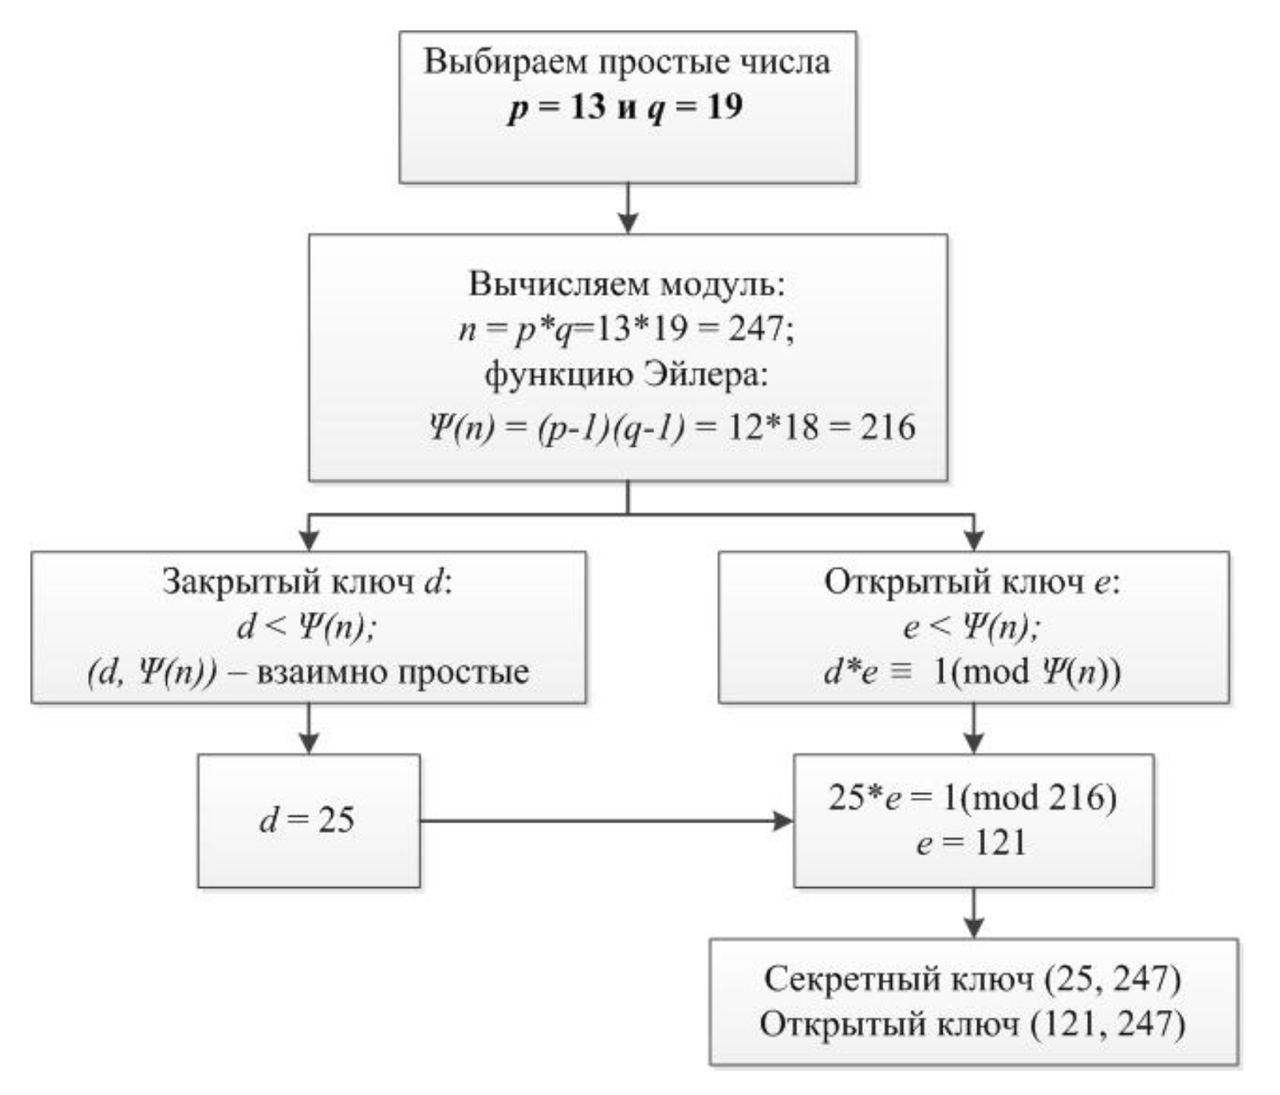
\includegraphics[width=1.0\linewidth]{../img/rsa_keygen.jpeg}
	\caption{Общая схема реализации алгоритма генерации ключей RSA}
	\label{img:rsa_keygen}
\end{figure}

\newpage

\subsection{Цифровая подпись}

На рисунке \ref{img:sign} представлена общая схема алгоритма электронной подписи и проверки электронной подписи.

\begin{figure}[!htb]\centering
	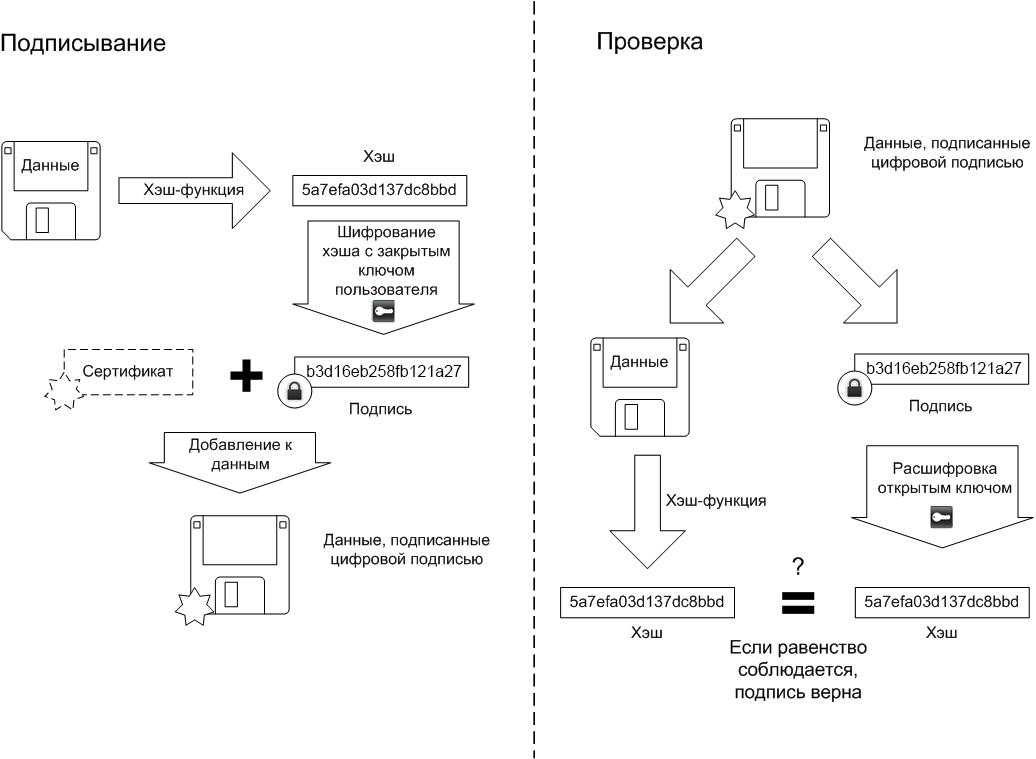
\includegraphics[width=0.75\linewidth]{../img/common.png}
	\caption{Общая схема алгоритма электронной подписи и проверки электронной подписи}
	\label{img:sign}
\end{figure}
